%%%%%%%%%%%%%%%%%%%
%  placeholders
%%%%%%%%%%%%%%%%%%%

% chair name not allowed at Department of Informatics
% remove \phantom{} if you want the chair name on the cover
\newcommand{\chair}{\phantom{Lehrstuhl f\"ur Musterverfahren}}
\newcommand{\faculty}{Department of Informatics}
\newcommand{\uni}{Technical University of Munich}
\newcommand{\studycourse}{Informatics: Games Engineering}

\newcommand{\authorname}{Jakob Raith}
\newcommand{\city}{Munich}

\newcommand{\worktype}{Master's Thesis in \studycourse}
\newcommand{\titleFirstLanguage}{Information Flow in Distributed Multi-Agent Systems as a Game Mechanic for Immersive Story Worlds}
% German & English needed at Department of Informatics
\newcommand{\titleForeignLanguage}{Informationsfluss in verteilten Multiagentensystemen als Spielmechanik für immersive Geschichtswelten}

\newcommand{\supervisor}{Prof. Gudrun Klinker, Ph.D.}
\newcommand{\advisor}{Daniel Dyrda, M.Sc.}

% set date manually or use \today
\newcommand{\submissionDate}{\today}



%%%%%%%%%%%%%%%%%%%
%    settings
%%%%%%%%%%%%%%%%%%%

% quick settings
\def\printstyle{twoside} % set to {twoside} for printing, else {oneside}
%\def\monochromeCover{} % uncomment if you prefer a black TUM logo on the cover
\def\monochromeCoverInside{} % uncomment if you prefer a black TUM logo on the inside cover page

% complete settings & packages: see settings.text
%%%%%%%%%%%%%%%%%%%
% essentials
%%%%%%%%%%%%%%%%%%%

% use the scrbook KOMA document class
\documentclass[	pdftex, 		%
		a4paper, 		% DIN A4 format
		titlepage,		% separate title page
		%draft,			% draft version, no figures in PDF!
		final,			% final version
		\printstyle ,		% see \def in main document (oneside or twoside)
		11pt,			% font size
		DIV=calc,
]{scrbook}
						
\setkomafont{disposition}{\normalfont\bfseries}
\usepackage{scrhack}

% page geometry - define custom if needed...
\def\coverborderleft{20mm} % needed for title page - update: Druck mit Pappumschlag braucht's eher nicht
\usepackage[left=30mm , right=30mm, top=30mm, bottom=30mm]{geometry}

% typesetting
\usepackage{palatino} 				% Palatino font with sans-serif \sffamily Helvetica
\usepackage[utf8]{inputenc} 			% Umlaute
\usepackage[T1]{fontenc}			% extended character set
\parindent0pt           			% no indentation of the first line
\parskip1ex             			% gap between paragraphs
\usepackage{setspace}				% package for line spacing settings
\singlespacing					% 1,0
%\onehalfspacing				% 1,5
%\doublespacing					% 2,0

% language for automated stuff, like "List of Figures" or "Abbildungsverzeichnis"
\usepackage[english]{babel}
%\usepackage[german=quotes]{csquotes} % Deutsche Anführungszeichen

% BibTex
%\usepackage{natbib}
%\bibliographystyle{plain}
\usepackage[style=numeric,backend=biber]{biblatex}
% add defernumbers=true

%%%%%%%%%%%%%%%%%%%
% custom cite game command
%%%%%%%%%%%%%%%%%%%
\DeclareCiteCommand{\citegame}
{\boolfalse{citetracker}%
	\boolfalse{pagetracker}%
	\usebibmacro{prenote}}
{\ifentrytype{software}{%
		\printfield{title}%
		\setunit{\addspace}%
		\printtext[parens]{%
			\printnames{author}%
			\setunit{\addcomma\space}%
			\printfield{year}}}{\GenericError{}{Not a game entry}{}{}}}
{\multicitedelim}
{\usebibmacro{postnote}}


%%%%%%%%%%%%%%%%%%%
% figures & co
%%%%%%%%%%%%%%%%%%%

% graphics and figures
\usepackage{graphicx, tikz, pgfplots}
\graphicspath{{images/}} % additional path(s) for loading images
\usepackage{rotating} % needed for \begin{sidewaysfigure} ... 

% insert PDF files
\usepackage{pdfpages}
% settings for PDF Pages to accept additonal versioned PDF files
\pdfminorversion=6
\pdfcompresslevel=9
\pdfobjcompresslevel=9

% define custom colors
\usepackage{xcolor}
\definecolor{gray1}{gray}{0.92}
\definecolor{darkgreen}{rgb}{0,0.5,0}
\definecolor{urlLinkColor}{rgb}{0,0,0.5}
\definecolor{LinkColor}{rgb}{0,0,0}
\definecolor{ListingBackground}{rgb}{0.85,0.85,0.85}

\usepackage{color}
\definecolor{LinkColor}{rgb}{0.1,0.1,0.1}
\definecolor{ListingBackground}{rgb}{0.98,0.98,0.98}
\definecolor{gray}{rgb}{0.4,0.4,0.4}
\definecolor{darkblue}{rgb}{0.0,0.0,0.6}
\definecolor{cyan}{rgb}{0.0,0.6,0.6}



%%%%%%%%%%%%%%%%%%%
% layout tools
%%%%%%%%%%%%%%%%%%%

% for \textblock on title page
\usepackage[absolute]{textpos}
%\setlength{\TPHorizModule}{1mm}
%\setlength{\TPVertModule}{\TPHorizModule}

% TUM Corporate Design definitions taken from official templates (tum.de/cd)
\newcommand{\UniversitaetLogoBreite}{19mm}
\newcommand{\UniversitaetLogoHoehe}{1cm}
\definecolor{UniversitaetFarbe}{RGB}{0,101,189}

% blindtext generator
%\usepackage{lipsum}

% advanced conditionals
\usepackage{pdftexcmds}


%%%%%%%%%%%%%%%%%%%
% math
%%%%%%%%%%%%%%%%%%%

\usepackage{amssymb}
\usepackage{amsmath}
% custom argmin, argmax
\newcommand{\argmax}[1]{\underset{#1}{\operatorname{arg}\,\operatorname{max}}\;}
\newcommand{\argmin}[1]{\underset{#1}{\operatorname{arg}\,\operatorname{min}}\;}



%%%%%%%%%%%%%%%%%%%
% code listings
%%%%%%%%%%%%%%%%%%%

\usepackage{listings}
\lstloadlanguages{TeX, C++, XML, Matlab, Java, Python, C} % add languages if needed 
\lstset{%
	language=[LaTeX]TeX,     %
	numbers=left,            % line numbers left
	stepnumber=1,            % number every line
	numbersep=5pt,           % distance of line numbers to the code
	numberstyle=\tiny,       % size of the line numbers
	breaklines=true,         % break lines if necessary
	breakautoindent=true,    % indent lines after line breaks
	postbreak=\space,        % line break at spaces
	tabsize=2,               % size of tab indentation
	basicstyle=\small\ttfamily,
	showspaces=false,        % don't show spaces
	columns=fullflexible,
	showstringspaces=false,  % ...also not in 'strings' / "strings"
	extendedchars=true,      % show all Latin1 chars
	backgroundcolor=\color{ListingBackground} % background color of the listing
}

% captions for listings
\usepackage{caption}
\DeclareCaptionFont{white}{\color{white}}
\DeclareCaptionFormat{listing}{\colorbox[cmyk]{0.43, 0.35, 0.35,0.01}{\parbox{\textwidth}{\hspace{15pt}#1#2#3}}}
\captionsetup[lstlisting]{format=listing,labelfont=white,textfont=white, singlelinecheck=false, margin=0pt, font={footnotesize}}



%%%%%%%%%%%%%%%%%%%
% header & footer
%%%%%%%%%%%%%%%%%%%

\usepackage{fancyhdr}
\pagestyle{fancy}
\fancyhead{}
\fancyfoot{} 
\renewcommand{\headrulewidth}{0.4pt} % line for header - 0.0pt = no line
\renewcommand{\footrulewidth}{0.0pt} % line for footer - 0.0pt = no line

\renewcommand{\chaptermark}[1]{\markboth{\thechapter\quad#1}{}}
\renewcommand{\sectionmark}[1]{\markright{\thesection\quad#1}}

\fancyhead[LO]{\textit{\rightmark}}	
\fancyhead[RO]{\textit{\thepage}}

\def\twoside{twoside} % macro needed
\ifx \printstyle \twoside
	% adapt footers and headers if two-sided
	\fancyhead[LE]{\textit{\thepage}}	
	\fancyhead[RE]{\textit{\rightmark}}
\fi



%%%%%%%%%%%%%%%%%%%
% hyperref
%%%%%%%%%%%%%%%%%%%

\usepackage[
	pdftitle={\titleFirstLanguage},
	pdfauthor={\authorname},
	pdfsubject={\titleFirstLanguage},
	pdfcreator={MiKTeX, LaTeX with hyperref and KOMA-Script based on template by Michael Grupp ( github.com/MichaelGrupp/TTT )},
	pdfkeywords={Abschlussarbeit, Thesis, TUM}, 
	pdfpagemode=UseOutlines,%                                  
	pdfdisplaydoctitle=true,%                                  
	pdflang=de%                                              
]{hyperref}

\hypersetup{%
	colorlinks=true,%        colored links without border
	linkcolor=LinkColor,%    
	citecolor=LinkColor,%    
	filecolor=LinkColor,%    
	menucolor=LinkColor,%    
	urlcolor=LinkColor,%     
	bookmarksnumbered=true%  
}
 



%%%%%%%%%%%%%%%%%%%
%  main document
%%%%%%%%%%%%%%%%%%%

\begin{document}

\frontmatter
% first part of document before actual content

\begin{titlepage}

% Dreizeiler:
\begin{textblock*}{\textwidth}(\coverborderleft, 2cm)%        	
    	\setlength{\baselineskip}{11pt}%
    	\ifx \monochromeCover \undefined
        	\textcolor{UniversitaetFarbe} { %
        	\fontsize{9}{11}\selectfont%
        	\sffamily \chair\\%
        	\sffamily \faculty\\%
        	\sffamily \uni }
    \else
        	\textcolor{black} { %
        	\fontsize{9}{11}\selectfont%
        	\sffamily \chair\\%
        	\sffamily \faculty\\%
        	\sffamily \uni }
    \fi
\end{textblock*}%

% TUM logo
\begin{textblock*}{\UniversitaetLogoBreite}[1,0](\paperwidth - 2cm, 2cm)%
		\ifx \monochromeCover \undefined
        	\includegraphics{images/TUM_Logos/TUM_blau.pdf}%
        \else
        	\includegraphics{images/TUM_Logos/TUM_schwarz.pdf}%
        \fi
\end{textblock*}%

% title text
\begin{textblock*}{\paperwidth - \coverborderleft - 2cm}(\coverborderleft , 8cm)% 
\raggedright %no hyphenation here
{\sffamily \Large \worktype}\\
{\sffamily \huge \titleFirstLanguage \par} %~\\[2mm]
\vspace{1cm}
\sffamily \Large \textbf{\authorname}\\
\end{textblock*}

~\\ % do not remove
\end{titlepage}
\begin{titlepage}
	\centering
	
	\ifx \monochromeCoverInside \undefined
		\includegraphics{images/TUM_Logos/TUM_blau.pdf}%
	\else
		\includegraphics{images/TUM_Logos/TUM_schwarz.pdf}%
	\fi
	\vspace*{20mm}
	
	\vspace{5mm}
	{\huge\MakeUppercase{\faculty}}\\
	
	\vspace{5mm}
	{\large\MakeUppercase{\uni}}\\
	
	\vspace{20mm}
	{\Large \worktype}
	
	\vspace{15mm}
	{\huge\bfseries \titleFirstLanguage}
	
	\vspace{10mm}
	{\huge\bfseries \foreignlanguage{ngerman}{\titleForeignLanguage}}
	
	\vspace{15mm}
	\begin{tabular}{l l}
		Author:          & \authorname \\
		Supervisor:      & \supervisor \\
		Advisor:         & \advisor \\
		Submission Date: & \submissionDate \\
	\end{tabular}
	
	\vspace*{20mm}
	
	\ifx \monochromeCoverInside \undefined
		\includegraphics{images/TUM_Logos/IN_blau.pdf}%
	\else
		\includegraphics{images/TUM_Logos/IN_schwarz.pdf}%
	\fi
	{}
\end{titlepage} % needed at Department of Informatics

\chapter{Eidesstattliche Erkl\"arung}
Ich versichere hiermit, dass ich diese Master's Thesis selbständig verfasst und nur die angegebenen Quellen und Hilfsmittel verwendet habe.
\\[1cm]
I confirm that this master's thesis is my own work and I have documented all sources and material used.
\\[6ex]

\city, \submissionDate

\vspace{1.5cm}
\rule[-0.2cm]{5cm}{0.5pt}

\textsc{\authorname} 

\chapter{Abstract}\label{Abstract}
The demand for high-quality video games is ever increasing. This entails every aspect of video game creation, such as graphic fidelity, sound design, gameplay innovation, or novel game design approaches. However, the ambition to tell truly interactive and dynamic stories is also a significant factor contributing to this trend. This thesis aims to create a novel game mechanic that supports narrative gameplay. The presented game mechanic is based on the exchange of information between the player and NPCs and among NPCs themselves. By modeling the NPCs as intelligent agents in a multi-agent system, techniques from this field are used to give the agents an autonomous behavior as they move through a 3D environment. A classification for different types of gameplay focusing on dynamic gameplay is created, and the developed prototype is compared to other current games in this classification. The resulting system creates a playground for varied narrative scenarios that are not previously defined by a game designer but can be explored by the player and are supported by the game systems.
\chapter{Acknowledgements}

I would like to thank Michael Grupp for this \LaTeX\ template.

%\lipsum[1-2]


\tableofcontents 


\mainmatter
% include chapter files here or write your text directly here

\chapter{Introduction}
Narrative heavy video games are ever more asked for by players. This is indicated by a report from WePC.com in which 73.55\% of people who play video games prefer single-player games over multi-player games~\cite{WePC2021}. This is, however, not to say that multi-player games can not focus on story. It is common though for single-player games to have a stronger focus on narrative. WePC.com further notes that gamers claim to play more video games because of the COVID-19 pandemic. Between March 23 and June 3rd 2020, the number of players has increased by 46\% in the United States, 41\% in France, 28\% in the United Kingdom and 23\% in Germany.~\cite{WePC2021}\\
The rise in interest in single-player games is also backed by Sony Interactive Entertainment. With 46\% of the console market, Sony is the leader of a \$58.6 billion industry segment.~\cite{Dealessandri2021} A supposedly leaked document mentioned in a Vice.com article reports, that the Sony consoles internal tracking tools found that PlayStation users spend more time offline than online on a regular basis~\cite{Klepek2020}. Finally, in an interview from March 2020, the head of PlayStation's Worldwide Studios, Hermen Hulst says that Sony is "very committed to quality exclusives. And to strong narrative-driven, single-player games."~\cite{Shuman2021} PlayStation Studios conists of 14 individual studios that focus on narrative driven single-player games~\cite{Sony2021}. All these commitments of the console industry leader to storytelling is a clear indicator, that the demand for games with narrative focus is present in the video game landscape.\\
Modern narrative games feature stories that rival movies in terms of production value. In May 2018, Eidos Montreal boss David Anfossi said, that the game \textit{Shadow of the Tomb Raider}~\cite{tombraider} cost \$75 - \$100 million just for production~\cite{Dring2018}. These more expensive games feature usually a very cinematic and action oriented storyline with well-known voice and performance actors. They are also usually quite linear in their structure and storytelling. Developers want to ensure that players actually see and experience the expensive set-pieces in the stories  which explains this more linear approach to storytelling.\\
But would interactive media like video games not profit from the potential of actually interactive storytelling? Players often wish for games to give them a lot of options in their interactions. "I want to be able to do whatever I want" is a request that comes up frequently when talking about open world games. Acclaimed game designer Sid Meier in his 2012 talk at the Game Developer Conference describes games as a "series of interesting decisions". He explains that through limiting and carefully crafting the actions a player can take, the gameplay becomes more compelling.~\cite{Dring2018}. So the argument can be made that "being able to do whatever I want" could actually be detrimental to the game experience. This argument can be extended into the story. Authored stories often follow rules of their respective culture's storytelling traditions. We perceive stories that deal with culturally relatable topics and follow familiar structural rules, more favorably.~\cite{Cooney2017}\\
But would players be able to make interesting narrative decisions naturally, given the option by a game that does not restrict interactions to an authored story? Does a video game story require an author at all? Can we  develop systems that take on that role? Could a game mechanic provide all necessary elements to satisfy narrative requirements? This thesis aims to explore not only what those requirements are and how they contribute to game stories, but also introduces a framework for game mechanics that allow the utilization of world state information for narrative purposes.\\
A story can be abstracted as numerous pieces of world information that are exposed to the person experiencing the story, in this case the player. If we have story that goes like "The knight slays the dragon." We now that the world consists of a knight, a dragon and the act of slaying the former. These pieces of information about the actors and acts in the world are then framed into a narrative structure - the story.\\
In this thesis, I developed a game mechanic based on modeling this kind of information into objects that exist in the game world. They are created by interacting with the world and are perceivable by agents that exist in the system next to the player. By allowing the non-player agents to react to newly learned information, the model creates an interplay among all agents in the system. The resulting game mechanic then is based on retrieving relevant information about characters or other objects in the game world and introducing new information as the player. This could even be used to create factually wrong information and thus allow the concept of lying to agents.\\
For the prototype game that was also developed as part of this thesis, I chose the following setup to showcase the game mechanic. The player controls a knight in a freely traversable 3D environment that represents a medieval kingdom. There are several key locations like a castle, a village or a farm that are inhabited by other \textit{non-player characters} (NPC) that represent the agents of the multi-agent system. The NPCs move around the kingdom and execute different tasks which bring them into contact with each other. When they interact they will also exchange information and thus learn new things about the game state. The player can also interact with characters and items and learn pieces of information. They can also engage in a conversation with NPCs and ask for or give out specific information. By adding quests to the game, a narrative framing exists that the player can use to motivate their actions.\\
Elevating the exchange of information in multi-agent systems to a core game mechanic, and allowing players to exploit the information flow is a novel system, that not many games support today. It is also, a step towards creating actual interactive story, because it allows for truly influencing the game world but still enabling developers to define rules for how agents and the environment reacts and thus enforcing a narrative structure.
\chapter{Theory} %25 pages
This chapter present the various fields of study, that were encountered or utilized while developing the game mechanic and its implementing prototype game. This includes fundamental story, game and quest theory, information theory, multi-agent systems, consensus protocols, emotion engines and inference engines.

\section{What is a story?}
There exist a multitude of definition on what a story is. Rayfield argues that story is a narrative item that exists throughout all cultures. He concludes that there exist a universal concept of a certain structure that listeners will recognize as a story. He limits this structure by degree of complexity and argues that listeners will only recognize the structure as story within certain minimal and maximal bounds of complexity. These bounds would then be the same across all cultures.~\cite{Rayfield1972} Scheub takes another approach and sees story more as "a means whereby people come to terms with their lives, their past; it is a way of of understanding their relationship within the context of their traditions. It is a means of accessing and valuing history: in the end story \textit{is} history."~\cite{Scheub1998} Lastly the Oxford Dictionary of Literary Terms more formally describes story as a set of events that are selected and arranged in a specific order and told by a narrator. The specific order of the events is called the plot.~\cite{Baldick1996} One thing that most definitions have in common however is that stories are an important tool for humans. Stories help us to interpret and process information and experiences. They enrich subjectively perceived facts and form them into each person's individual truth. This is the \textit{"meaning"} of a story. This "meaning-making" is also part of the psychological process in self-identification and the creation of memories~\cite{Flanagan1992}. Stories are furthermore an important factor in human communication, used as parables and examples to illustrate points. Storytelling was one of the earliest forms of entertainment.\\
When looking into definitions of what a story \textit{is}, the matter quite quickly goes into the area of what a story \textit{does}. I already mentioned how it is a vital tool for the human psyche but there are some more concrete functions that stories fulfill.

\subsection{Functions of Storytelling}
The motifs and contents of stories and the modes of narration are highly culturally individual aspects. The functions these elements serve though, can be found across all cultures. One example is to make one narration more understandable by putting it into relation with another story. This is commonly referred to as a metaphor. Now these relational stories do't have to be imaginary per se. They can be a retelling of events that have actually transpired an help underline the point of the narrator. On the far hand of abstracting stories to make a point is the very careful use of words to find an objective true transpiring of events. This is what happens in courtrooms. It is a retelling of events, but the order and selection is so careful, so meticulous, that an actual fair "true" story might be revealed.~\cite{Rigney1992}\\
As mentioned above stories and storytelling are used to share and interpret experiences. The human brain is evolutionary predisposed to process, store and recall memories in the form of stories~\cite{Wyer2014}. Humans think in narrative structures and mostly remember facts in the form of a story. Facts are smaller versions linked to a larger story, which supports analytical thinking.~\cite{Connelly1990} This makes storytelling such a great tool for teaching as well. There is research about how storytelling is a meaningful teaching method that can be applied in education to encourage the development of caring, empathy, compassion and to develop a deeper cultural understanding.~\cite{Davidson2004} It is not event solely the listening person who is learning from a story. Often the discovery of a personal meaning of a story is only made visible when telling a story. Thus also the storyteller can learn something new.~\cite{Doty2003}\\
This is applied in therapeutic storytelling, where through retelling experiences in story form, the storyteller attempts to better understand their own thoughts and situation. This can be supported by questions from a therapist who carefully steers the storyteller through their narration to pinpoint insights.~\cite{Lawless2001}\\
There are countless situations where we encounter storytelling precisely because we want to share experiences and emotions. Stories are used to inspire and motivate, to manage conflicts, for marketing or for political practice~\cite{Jameson2001}. These are all situations where the intent is separate from the story itself. Where we turn to storytelling because the human brain can process them so effectively. Another aspect is however when we tell stories for the story's sake.


\subsection{The Appeal of Stories}
I have now established that there is a difference between the intention of storytelling itself and utilizing it for another purpose. The difference is that we do not enter a courtroom to tell or listen to a story. We do so to find the truth. The past has simply show us that the careful recounting of events combined with precise inquiry, has proven a good way to do so. So when we do not tell stories as a means of achieving another intention, we also share them just because they are stories. For this we can take on both positions, that of the narrator or the listener. Again, a multitude of situations presents itself for these applications. We listen to bedtime stories that our elders tell us. We tell a funny anecdote to our friends on a night out. Humans have created whole industries around the consumption of stories. We read books to immerse ourselves into stories, we watch movies or shows and we play video games. The fact that so much of our time is willfully spent listening to, watching or interacting with stories, must mean that there is something worthwhile there. The mere consumption of a narration seems to be satisfying in itself.\\
When we hear stories, the brain releases the hormone Oxytocin. This hormone heightens feelings of trust, empathy and compassion. It positively influences social behavior and helps us to feel more connected to others.~\cite{Gottschall2012} Humans are inherently social beings. We want to connect to others around us. We try to create situations and use known cultural signals to connect on a non-verbal level. Humans mimic body language, laugh more in social situation than alone or use physical contact to communicate.~\cite{Frith2007}\\
When we hear a story, the brain is enabled to form connections to the people who listen to the story with us, to the narrator and to the characters in the story. Communication is a shared activity resulting in a transfer of information across brains. Research shows that during successful communication, the brains of both the speaker and the listener shows common, temporally linked, response activities. When we hear a story, our brain mirrors activities in the sensory center of the storyteller.~\cite{Stephens2010} This attempt to sync brain activity is a deeply social connection. It also means, that when we hear an enjoyable story, the brain behaves as if we would experience it ourselves.

\subsection{Stories in Media}

\subsection{Expectation \& Feedback}

\subsection{The optimal Experience}

\subsection{Quests}
% Story	- 3 pages
	% Appeal
	% Stories in media
	% Feedback - expectation
	% optimal experience
	% Quests
\section{Concretizing Information}
% Information - 3 pages
	% Types of Data
	% Mutation
\section{Game Mechanics}
% Game Mechanic - 3 pages
	% emergent
	% multiplicative game design
\section{Multi-Agent Systems}
% Agents - 3 pages
	% Games as multi agent systems
\section{Consensus}
% Consensus - 3 pages
	% Quorum
	% Proof of Personhood
\section{A Heuristic for Information}
% Heuristic for story relevant information 3 - pages
	% MapReduce
\section{Related Work}
\subsection{Emotion Engines}
% Related Work - Emotion Engines - 3 pages
\section{Inference engines}
% Inference engines - 3 pages
\chapter{Implementation} % 25 pages
The following chapter describes the prototype game I created as part of this thesis. I explain how I applied the concepts and research introduced in the previous chapter.\\
The game simulates a small medieval kingdom and its inhabitants. The player controls a knight who is sent on a quest by the queen. The king is missing and the player shall return the king to the castle. The player can move around and interact with non-player characters (NPCs) and some key items. First I will introduce the \textit{Information Model}, that I created to define information in the game. Then I will go into detail about the \textit{agents}, that inhabit and exist in the game world. After that, I will describe the \textit{game world} itself followed by a \textit{gameplay} description. Then I will focus on the \textit{dialogue feature} and how information can be retrieved and introduced into the system. Following that I will give an explanation of how narrative is introduced using \textit{quests}. Additionally, I will provide the concrete implementations of both the information \textit{heuristic} and the \textit{consensus protocol}. The chapter will be closed off, by discussing the \textit{narrative implications} of the described gameplay.
\section{Technology}
Before I go into detail about the game logic, I want to explain my choice of development environment. For the prototype game I chose the Unity engine developed by Unity Technologies~\cite{Unity2021}. This choice was made because I have multiple years of experience with the Unity engine and it allows for fast prototyping that is easy to iterate upon. Unity is widely used across the video game industry, has an active developer community and is well documented. The programming language for Unity is Microsoft C\# with the .NET framework, which I have also many years of experience with. All assets that are used in the prototype game are either purchased or free to use. All asset creators are properly credited in the prototype.
\section{Information Model}
At the center of the game mechanic created for this thesis, is the \textit{Information Model}. I propose a conceptional model for information objects that encapsulate statements about semantic and factual game world data (see \ref{section:info}). The statements encapsulated in an \verb|Information| object is primarily characterized by its \textit{Verb}. The verb is the main indicator of the assertion of the information content. Every information object also contains a \textit{Subject} which denotes who or what the information statement is concerned with. The third part of the information is dependent on the verb and can either be an \textit{Object}, an \textit{Adjective} or a \textit{Location}.
Thus every information object $I$ consists of a triple of information elements:
\begin{center}
	$I \coloneqq \{s, v, x\}$ 
\end{center}
Where $s$ is the subject, $v$ is the verb and $x \in \{\textit{Object, Adjective, Location}\}$ depending on the verb. Figure~\ref{fig:informationCD} shows the class diagram for the \verb|Information| class. Although the elements of an \verb|Information| object refer to actual game objects in the game world, this link is purposely severed when an \verb|Information| object is created. This is done, so that the information statement is actually just that and has no exploitable connection to other objects anymore. Thus the \textit{Information Model} and the programming interface remain decoupled which allows for a more accurate simulation.\\
The \verb|Information| class also implements the \verb|IMutatable| interface which only declares the function \verb|Mutate|. This function should reduce the accuracy in the statement by reducing the accuracy in any of the statement components every time it is called.
\begin{figure}
	\centering
	\includegraphics[width=0.3\textwidth]{InformationCD}
	\caption{Inheritance diagram of the Information class}
	\label{fig:informationCD}
\end{figure}
\subsection{Verbs}
Verbs in the \textit{Information Model} come in three types:
\begin{itemize}
	\item \textbf{IS}: Creates information statements about the \textit{state} of a subject of the form "\textit{Subject} \verb|IS| \textit{Adjective}".
	\item \textbf{HAS}: Creates information statements about a possessive relationship between subject and object of the form "\textit{Subject} \verb|HAS| \textit{Object}".
	\item \textbf{AT}: Creates information statements indicating the location of a subject of the form "\textit{Subject} \verb|AT| \textit{Location}". The \verb|AT| type presents a special form of the \verb|IS| type, but in the context of a traversable 3D world, locations represents such an important piece of state, that its own information type is justified.
\end{itemize}
\textit{Verbs} are instances of the \verb|Verb| enumeration. The constructors in the \verb|Information| class are designed in such a way, that the verb is set by the constructor and there exist multiple overloads to create the different types of information objects (Listing \ref{listing:information}).
\begin{lstlisting}[
	caption={Information class constructors},
	label={listing:information}
	]
	public Information(Agent agent, Item object)
		=> (Subject, Verb, Object, Adjective, Location, Not) =
		(agent.InformationSubject, InformationVerb.Has, object.InformationSubject, null, null, false);
	
	public Information(WorldObject subject, InformationAdjective informationAdjective)
		=> (Subject, Verb, Object, Adjective, Location, Not) =
		(subject.InformationSubject, InformationVerb.Is, null, informationAdjective, null, false);
	
	public Information(WorldObject subject, InformationLocation informationLocation)
		=> (Subject, Verb, Object, Adjective, Location, Not) =
		(subject.InformationSubject, InformationVerb.At, null, null, informationLocation, false);
\end{lstlisting}
This way \verb|Information| objects can be created with only the content in mind, and the constructor sets up the object correctly for usage.
\subsection{Subjects}
As mentioned, every piece of information contains a \textit{subject}. They represent the concerning entity of an information statement. A \textit{subject} is an instance of the \verb|InformationSubject| class that conceptually either represents an \verb|Agent| or an \verb|Item|, both of which inherit from the \verb|WorldObject| class.\\
What exact type of object a \textit{subject} is in a given \verb|Information| object, is again dependent on the \textit{verb}. For example there can be no information of the form "\textit{Item} \verb|HAS| \textit{Agent}" because an item cannot own an agent. The constructors for \verb|Information| objects make sure that no erroneous object can be created.\\
\textit{Subjects} consist  of a textual name that denotes the \textit{subject} and two boolean values that state whether the \textit{subject} is an agent or not and whether it is a unique object, which is important for items (Figure~\ref{fig:subjectCD}).
\begin{figure}
	\centering
	\includegraphics[width=0.6\textwidth]{SubjectCD}
	\caption{Inheritance diagram of the InformationSubject class}
	\label{fig:subjectCD}
\end{figure}
\textit{Subjects} also have a \verb|Mutation| object attached that is responsible for decaying the accuracy of the \textit{subject}. I give a detailed explanation of mutations in Section~\ref{section:mutation}.
\subsection{Adjectives}
An \textit{adjective} represents a detail or characteristic of a \textit{subject's} state. The can be arbitrarily defined by a developer. They represent the properties of a \textit{subject}. \textit{Adjectives} are instances of the \verb|InformationAdjective| class (Figure~\ref{fig:adjectiveCD}). In the \textit{Information Model} there are two differentiable types of \verb|InformationAdjective| objects:
\begin{itemize}
	\item \verb|InformationProperty|: Represents factual information about a \textit{subject}. For example "\textit{Agent} \verb|IS| \textit{alive}." is a factual piece of information that can be either true or false.
	\item \verb|InformationOpinion|: Represents statements about a \textit{subject's} state that are influenced by information holder's relationship to the \textit{subject}. For example the statement "\textit{Agent} \verb|IS| \textit{dangerous}." can be true for one agent but false for another.
\end{itemize}
This distinction is introduced so that conceptually there can be a difference between facts and opinions that someone has about any \textit{subject}.\\•
An \verb|InformationAdjective| consists of the textual \textit{Characteristic} and a list of \textit{contradictions}. The contradictions are other \textit{adjectives} that are conflicting with the \textit{adjective} they are attached to. A simple example would be the two information statements  "\textit{Agent} \verb|IS| \textit{alive}." and  "\textit{Agent} \verb|IS| \textit{dead}.". Both cannot be true at the same time. Therefore, each \textit{adjective's} contradictions list contains the respective other. When an agent learns a new information that contains an \textit{adjective}, they check the \textit{adjective's} contradictions and resolve any conflicts.\\
At the start of the game, an initial list of \textit{adjectives} that exist in the world is created. After that, the contradictions lists are created and attached to each \textit{adjective}.
\begin{figure}
	\centering
	\includegraphics[width=0.8\textwidth]{AdjectiveCD}
	\caption{Inheritance diagram of the InformationAdjective class}
	\label{fig:adjectiveCD}
\end{figure}
\subsection{Locations}
As mentioned before, a \textit{location} is a special kind of \textit{object} for the \verb|AT| information type. In a 3D game world that is driven by a multi-agent system, agents need to move around. For that the \verb|InformationLocation| class attaches a position in the world to the information so that agents can retrieve an actual location from the information statement.\\
A \textit{location} also has a \verb|Mutation| object attached to it, so its accuracy can be reduced. Other than that, the \verb|InformationLocation| has only a textual name and the 3D position as a public interface.
\begin{figure}
	\centering
	\includegraphics[width=0.6\textwidth]{LocationCD}
	\caption{Inheritance diagram of the InformationLocation class}
	\label{fig:locationCD}
\end{figure}
\subsection{Mutation}
\label{section:mutation}
To simulate the decay of information and agents forgetting details, the \textit{Information Model} implements a \textit{Mutation} functionality. \verb|InformationSubject| and \verb|InformationLocation| objects have an object of the \verb|Mutation| class. These represent a hierarchy of less precise information values. Every \verb|Mutation| object has a reference \verb|ParentMutation| that points to a \verb|Mutation| object that holds the next less precise information value.\\
As an example, we assume the \verb|InformationLocation| $l$ with the name value "\textit{Village Square}". The \verb|Mutation| object can point to a less precise information value "\textit{Village}" which in turn points to an information value "\textit{Somewher in the South}". This way when $l$ is mutated once, its name value will be "\textit{Village}" and if mutated again will decay to "\textit{Somewhere in the South}" where it will remain.\\
This mechanic allows for agents to slowly forget about details in their information statements which makes the collection of memories more chaotic over time.\\
The values for the mutation hierarchy are set by the developer before the game starts.\\
The \verb|Mutate| function in the \verb|Information| class that is provided by the \verb|IMutatable| interface triggers the mutation of any of its statements' components.
\section{Agents}
In any multi-agent system, the central component are of course the agents. In the prototype game, those agents represent the NPCs who live in the game world or the player (Figure~\ref{fig:agentCD}). The only difference is that the player agent is controlled by the player instead of the game. But for the NPCs, there is no difference between the player agent or any other NPC. In the following I will generally talk about NPCs as agents for better understanding of the conceptual implications in a multi-agent system. Agents move around in the world to perform actions, exchange information and change their state depending on what they learn.
\begin{figure}
	\centering
	\includegraphics[width=0.6\textwidth]{AgentCD}
	\caption{Inheritance diagram of the Agent class}
	\label{fig:agentCD}
\end{figure}
The \verb|WorldObject| class is the parent class for both \verb|Agent| and \verb|Item| classes. I represents physical entities that exist as part of the multi-agent system. \verb|WorldObject| itself is a child class of Unity's \verb|MonoBehaviour| class which is the base class of all game objects managed by the Unity engine.\\
All \verb|Agent| instances inherit the members of their parent classes and thus have a textual identifier \textit{Name}, a \textit{Location} to denote the object's current location, exposed properties to set up the \textit{InformationSubject} and an integer value \textit{WorldImportance}. This value is important for the information heuristic for believability which is described in section %TODO add ref to heuristic.
\textit{WorldImportance} indicates the initial interest a piece of information gets through the involved object. This interest can be positive or negative. A piece of information about the castle might have high positive value, since the castle is an important place in the kingdom. Information about an enemy bandit however, will have a negative number, as people are afraid of the bandits. These values should be an objective measure of an object's interest value. Subjective views from the agents are taken into account when the heuristic is calculated.\\
The important properties of the \verb|Agent| class are the \textit{Inventory} which stores items in the agent's possession, \textit{Acquaintances} contains other agents that have interacted with the object, \textit{ImportantPeople} are agents that have a close relationship with the object like friends or loved ones and \textit{Quests} which is a list of objectives the agent has. Through the \textit{ImportantPeople} property, certain agents can be treated differently and more favorably than others. This allows the introduction of a social network component into the multi-agent system.\\
The boolean values \textit{IsSeeing} and \textit{IsHearing} allow to determine what kind of information the agent is able to "sense" respectively.\\
The heart of the game mechanic is the \textit{Memory} property. It is an \verb|InformationManager| object. As the name implies, it stores, processes and manages all the incoming pieces of information.\\
The different actions an agent can execute are also defined here. This includes interacting with other agents, picking up and dropping items or attacking agents.
\subsection{NPC}
The \verb|NPC| class is a child class of the \verb|Agent| class and defines additional properties and functions that are unique only for NPCs.\\
This includes a \textit{Routine} property which is a list of behaviors the agent will execute one after another to simulate a daily life of a human. When they reached the end of their routine, they will start again from the beginning.
\subsection{Player}
In the scope of this thesis the \verb|Player| class behaves very similar to other agents. It has components attached that enable input to control the player agent. It needs its own class, so that developers can differentiate between NPCs and the player. This is necessary as the agents don't might want to behave differently when interacting with the player agent to expose more information to the actual player in front of the screen. For example when a dialogue is started, an NPC will not simply send information and continue with its routine, but it will pause and the dialogue interface will be opened where the information exchanged is controlled by the player.
\subsection{Behavior}
In order for the intelligent agents to move, interact and follow their objectives, I defined multiple behaviors that allow them to perform actions (Figure~\ref{fig:behaviorCD}). The following behavior classes exist:
\begin{itemize}
	\item \verb|ExchangeInformationBehavior|: This behavior allows two agents to engage in an exchange a piece of information. They choose which information to send each other based on the information heuristic.
	\item \verb|SendInformationBehavior|: As a child class of \verb|ExchangeInformationBehavior|, this behavior selects a random agents from the list oof \textit{ImprotantPeople} and sends them a piece of information also based on the information heuristic. This behavior can be interpreted as "sending a message" to a distant friend. I implemented this so that information would also reach farther parts of the world eventually.
	\item \verb|WalkBehavior|: This simply allows the agent to move to a specified location in the world.
	\item \verb|TalkBehavor|: This would allow NPCs to stop the player and engage in a conversation with them. In the prototype game this behavior is never used and it is only the player who can initiate a  conversation.
	\item \verb|WaitBehavior|: To simulate NPCs that are waiting or "doing nothing" for a specified time, I implemented this behavior. It is mostly to make the simulated behavior look more realistic and have NPCs stand in a place for a while.
	\item \verb|PickUpBehavior| and \verb|DropBehavior|: These two are implemented to let NPCs pick up a specified item in the vicinity or drop it in font of them respectively.
\end{itemize}
\begin{figure}
	\centering
	\includegraphics[width=1.2\textwidth]{BehaviorCD}
	\caption{Inheritance diagram of the AgentBehavior class}
	\label{fig:behaviorCD}
\end{figure}
The parent \verb|AgentBehavior| class is an abstract class and declares functions for starting, interrupting and resuming a behavior. Additionally it declares the function \verb|IsBehaviorFinished| to check if the behavior is completed. This simple setup of behavior allows for easy extension of the capabilities of agents.
\subsection{Information Manager}
At the heart of the agents' logic is the \verb|InformationManager| class. It provides all the necessary functions to add, manage and process incoming \verb|Information| objects for an agent. Its main task are adding new pieces of information to the memory and evaluating them on a regular basis to update the information heuristic values.\\
It manages the different pieces of information with lists of \verb|InformationContext| objects. Those are objects that pack an \verb|Information| object with contextual data about how the information was received. The context object stores how many times the information was received already by distinct agents, who it was received from, the time since it was last received and current values for believability and information heuristic.\\
The \textit{Information Manager} provides two lists of \verb|InformationContext| objects to manage its memories:
\begin{itemize}
	\item \textit{Speculative Memory}: the speculative memory stores every piece of information that an agent receives. It is a list of unconfirmed information that needs to be evaluated before it can be trusted. Only information that the agent did not perceive itself but was given to it by others, is considered speculative.
	\item \textit{Stable Memory}: confirmed or trusted information is stored in the stable memory. Everything an agent learns by its own senses like seeing, hearing or otherwise witnessing goes directly to the stable memory. If information is received via another agent, it needs to be verified through believability before it is transferred from the speculative memory to the stable memory. When an agent evaluates the information stored in its memory, it also updates believability values for every piece of information. This value is closely tied to the information heuristic. If the believability of an information is above a certain threshold, it is transferred to the stable memory and if it falls under the threshold, it is sent back to the speculative memory.
\end{itemize}
This structure, of speculative and stable memory is taken from high availability backup systems. A process called chain replication uses a similar technique, where any change to the system is put into a speculative history until all nodes in the backup change have confirmed it. After that it is transferred through all nodes again, but in a stable history. When all nodes have confirmed the change in the stable history, the update was successful.~\cite{Van2004}\\
Although agents are only a single node, I tried to replicate this confirmation methodology with the speculative and stable memories.
\section{Game World}
The agents in the prototype game live in an environment. The environment in the prototype game is \textit{inaccessible}, \textit{deterministic}, \textit{static} and \textit{discrete}. It is inaccessible because agents learn of changes in the environment state only when they perceive or receive information about them, not as they happen. It is deterministic because every change an agents performs on the environment's state is known beforehand. The environment is static because the topology and and structure does not change in this prototype and it is discrete because the space agents can move in is limited.\\
In the prototype game, the environment for the multi-agent system is the game world. I created a 3D world that contains interesting and memorable locations that agents can move around in. I recreated a small kingdom with several settlements where different agents live and go about their day. The key locations are \textit{the village}, \textit{the castle}, \textit{the sawmill}, \textit{the forest}, \textit{the lake}, \textit{the farm} and \textit{the enemy camp}~\ref{fig:gameWorld}.
\begin{figure}
	\centering
	\includegraphics[width=1\textwidth]{GameWorld}
	\caption{An overview of the game world.}
	\label{fig:gameWorld}
\end{figure}
The landscape is filled with paths and landmarks to make orientation easier and guide the player between the locations.\\
I chose a medieval kingdom for my environment since it is a well understood and established context for video game worlds. Ford in his work about medieval towns in single player games describes how the boundaries between village and nature are also boundaries between the home and the frontier, the old and the new, the familiar and the unknown. This does not only relate to classic narratives about heroes venturing out into the wild, but also says interesting things about this dichotomy in game worlds. Video games often contextualize towns and nature through their mechanics. There are games for examples where you cannot use your weapons while inside a town or city. They also very often serve as quest hubs or quest destinations. This means that the borders define on a mechanical level what the player is allowed to do. Much like with real-world definitions of borders, this might say more about the player and their position in the game world than it does about the city ot town itself.~\cite{Ford2019}
\section{Gameplay}
I have touched previously upon what the player interactions are that form the gameplay of the prototype game. Players control a knight in the kingdom who sets out to go on quests and adventures in the kingdom (Figure~\ref{fig:gameplay}). The player controls the movement of the knight and can talk to NPCs and interact with key items. If the player picks up a weapon, the character is able to attack other agents.\\
The novel game mechanic this prototype now presents and that is the topic of this thesis is more about the \textit{How} than the \textit{What}. Initially the player character is given a quest to return the king back to the castle. That is all the information the player is given who is now free to roam the game world to try and reach this goal.\\
Though talking to NPCs and learning new information about the world, the player can find clues that help them reach their goal. Where exactly is the king? Is he guarded by a monster? How can I defeat the monster? NPCs can give pieces of information that let the player step by step deduce an answer to this question.\\
Or the player can go a completely different route. By talking to NPCs they can introduce new or even wrong pieces of information into the world. Could I convince enough people that I am the king? And if someone would tell the queen, would she believe I am the king? And would that allow me to go back to the castle and thus achieve the goal?\\
The systems that I have created for this prototype allow for varied and interesting solutions to quests even for the little amount of content that is in the prototype.
\begin{figure}
	\centering
	\includegraphics[width=1\textwidth]{Gameplay}
	\caption{A sample gameplay scene.}
	\label{fig:gameplay}
\end{figure}
\section{Dialogue}
The main way to purposely learn and give out information in the game is to talk to NPCs. For that I have created a dialogue system that let's you either receive a random information from a NPC, ask a specific question or make a  statement on your own.\\
I used Yarn Spinner from Secret Lab to create the dialogue~\cite{Secret2021}. It is a lightweight tool that comes with a Unity plug in and allows for branching node-based dialogue and supports variables and simple logic in its dialogue files.\\
Yarn Spinner comes with an editor that easily allows developers to set up and write complex and branching dialogue files.
\begin{figure}
	\centering
	\includegraphics[width=1\textwidth]{Yarn}
	\caption{The NPC Yarn dialogue file}
	\label{fig:yarn}
\end{figure}
\subsection{Questions}
Allowing the player to ask questions about specific game objects is much more goal oriented that randomly hoping for useful information to happen upon the player. The dialogue interface allows the player to create questions from a question verb, an information verb and an object(Figure~\ref{fig:question}). The question verbs \textit{Who}, \textit{What}, \textit{Where} and \textit{How} indicate whether the expected answer will be a NPC name, an item, a location or an adjective. The question object contains options depending on the selection of question verb and information verb. If the NPC has an information that matches the question requirements, it will tell it to the player.
\begin{figure}
	\centering
	\includegraphics[width=1\textwidth]{Question}
	\caption{Posing a statement to an NPC.}
	\label{fig:question}
\end{figure}
\subsection{Statements}
This allows the player to create new information based on object they have encountered while playing. In the dialogue interface, the player can create information statements like they are defined in the \textit{Information Model}(Figure~\ref{fig:statement}). The selected verb will define what options are available for information subject and information object. The available subjects and objects depend on the NPCs, items and locations, the player has encountered so far. Only adjectives are universally known by all agents as they do not represent things in the world but rather concepts.\\
If the information statement is well-formed according to the \textit{Information Model}, the newly created information will be transmitted to the NPC as if any other agent would have told to it.\\
The functionality to create any information from known components creates the ability to lie for the player which creates interesting gameplay implications.
\begin{figure}
	\centering
	\includegraphics[width=1\textwidth]{Statement}
	\caption{Asking a question to a NPC.}
	\label{fig:statement}
\end{figure}
\section{Inference}
To simulate the flow and creation of information more realistically in the NPCs, they can also deduce new Information from the ones they have. These deductions are based on rules that are globally defined and represent a form of cohesive causal understanding of the game world. To define such rules, there is the \verb|InferenceRule| class. It consists of a \verb|BoolExpression| object that defines the rule and a list of \verb|Information| objects that define the consequences or outcomes if the rule applies.\\
The \verb|BoolExpression| object holds \verb|Information| objects and is chained together with other \verb|BoolExpression| objects by logical operators to create the rule. Listing~\ref{listing:rule} defines the following rule for any agent $X$:
\begin{center}
	\textit{isArmed}$(X) \wedge $ \textit{isEnemy}$(X) \Rightarrow $ \textit{isDangerous}$(X)$ 
\end{center}
\begin{lstlisting}[
	caption={Creating an inference rule with consequences},
	label={listing:rule}
	]
	var rule = new InferenceRule(new BoolExpression(new Information(_player, WorldAdjectives[Adjectives.Armed]))).And(new BoolExpression(new Information(_player, WorldAdjectives[Adjectives.Enemy])));

	rule.Consequences = new List<Information> { new Information(_player, WorldAdjectives[Adjectives.Dangerous]) };
\end{lstlisting}
The variable \verb|_player| in the statement is just a placeholder and is replaced with different subjects during evaluation of the rule. For the scope of this thesis it made only sense to substitute for information subjects, since the \textit{Information Model} is structured in such a way, that the information statements say something about an information subject.\\
In order to evaluate such a rule, every agent has an \textit{Inference Engine} that allows them to to so. The \textit{Inference Engine} sees the agent's stable memories as its knowledge base. It goes through the rules and checks if the knowledge base of the agent satisfies the rule. If so, all the pieces of information that are defined in a rules's list of consequences is added to the stable memory of the agent(Listing~\ref{listing:evaluate}). This is repeated until no new information is added, since any new information could trigger another rule.\\
The \verb|SatisfiesKnowledgeBase| function recursively checks if a rule's \textit{Boolean Expression} applies to the agent's memories. A information's subject is selected as a candidate if the information matches the information in the \textit{Boolean Expression} in all components except for the subject.
\begin{lstlisting}[
	caption={Evaluating inference rules},
	label={listing:evaluate}
	]
	public void Evaluate(){
		foreach (InferenceRule rule in Rules){
			List<InformationSubject> candidates = SatisfiesKnowledgeBase(rule.Expression, new List<InformationSubject>());
			
			if (!rule.AppliesToSelf)
				candidates.Remove(KnowledgeBase.Owner.InformationSubject);
			
			if (candidates.Any()){
				candidates.ForEach(c =>{
					rule.Consequences.ForEach(r =>{
						r = new Information(c, r);
						KnowledgeBase.TryAddNewInformation(r, KnowledgeBase.Owner);
					});
				});
				Evaluate();
			}
		}
	}
\end{lstlisting}
This way agents can "reflect" on what they know and deduce new information.
\section{Heuristic}
% Heuristic 2
Each agent is able to subjectively evaluate the believability of pieces of information it has stored in its memory. A metric is needed to measure the believability of information. I approached this via the "interest" of an information. This means how special is a piece of information or how probable is it that a give information could be true. This depends on the "interest" of the involved information components. The information "\textit{Farmer} \verb|HAS| \textit{milk}" is much more probable or uninteresting" than the information "\textit{The king} \verb|HAS| \textit{the magical sword}". So by evaluating the components of the information and their relation to one another, a value for the "interestingness" of an information is calculated. I call this value \textit{Information Heuristic}.\\
The calculations for the \textit{Information Heuristic} are of course slightly different depending on types of the involved information components. The general idea is that the more "interesting" an information is, the higher its \textit{Information Heuristic} is. To make this value subjective to the agent, values that depend on the agent's experience or relation to involved agents is are taken into consideration.\\
The basic formula is as follows:
\begin{equation}
	h = h\ h'\ b\ n_i\sum_{a \in K}trust(a)
\end{equation}
with $K \coloneqq \{A \cap I\}$, where $A$ is the set of known associates of the agent and $I$ is the set of agents this information was previously received from.\\
The value $h'$ is the part of the heuristic that is dependent on the verb and the information components, $b$ is the previous believability of the information and $n_i$ is the number of times this information has already been received.\\
In other words, an information's heuristic is the product of itself with the component-dependent heuristic, the believability, the number of times it has been received and the sum of the trust values of known agents this information has been received from. \\
Now the component-dependent heuristic is another calculation heavy function. It differentiates between the verb and then in each case calculates the value differently depending on the components. If another agent is involved for example, the distance or degrees of separation between the bespoke agent and the receiver of the information is taken into account. The calculation is done using breadth-first search. This should reflect cases where information is received like "I heard from a friend of a friend...". The longer the distance, the less trustworthy the information. If the subject is a known associate, then the trust the agent has towards the subject is also considered. The number of other pieces of information the receiver has, concerning the subject is also used. This should reflect a familiarity with the subject.\\
If the subject of the information is an item, then not only is the uniqueness of the item in world relevant but also how unique the item is for the agent. This takes into account, whether the agent owns an item of the same type and how many other pieces of information it has that refer to an item of the same type. This again is to simulate how familiar the agent is with the bespoke item.\\
So now there is a value for every information an agent has, that says how "interesting" or "probable" that information is. To calculate the believability of an information, this heuristic is now put into context with every other information an agent has. I define the \textit{distance} between two pieces of information as the absolute difference between their heuristic values.\\
For the believability $b$ of a piece of information this results in:
\begin{equation}
	b = \frac{\sum_{i,j \in M, i \neq j} h(i)-h(j)}{n}
\end{equation}
In this formula, $n$ is the size of the stable memory and $M$ is the stable memory itself. The function $h$ is the heuristic function. This means the believability of an information is the average distance to every other information in the stable memory.\\
Since this is calculated for every information in the stable memory of every agent, this operation needs a lot of processing power. I implemented the MapReduce programming model to enable the distribution of these calculations. The prototype does not leverage the distribution itself since this was too big a task for the scope of the thesis, but the implementation is prepared to be used with little additional work (Listing~\ref{listing:map}). The \textit{Map} and \textit{Reduce} steps are marked with comments in the listing.
\begin{lstlisting}[
	caption={The MapReduce implementation for calculating believability},
	label={listing:map}
	]
public void UpdateBelievability(){
	List<InformationContext> data = GetAllMemories();
	
	// Map
	var distances = new List<List<float>>();
	
	for (int i = 0; i < data.Count; i++){
		distances.Add(new List<float>());
		for (int k = 0; k < data.Count; k++){
			Information i1 = data[i].Information;
			Information i2 = data[k].Information;
			if (!i1.Equals(i2))
				distances[i].Add(GetInformationDistance(i1, i2));
		}
	}
	
	// Reduce
	for (int i = 0; i < distances.Count; i++){
		if (ContainsStableInformation(data[i].Information) && distances[i].Any())
			GetStableMemory(data[i].Information).Believability = distances[i].Average();
		else if (ContainsSpeculativeInformation(data[i].Information) && distances[i].Any())
			GetSpeculativeMemory(data[i].Information).Believability = distances[i].Average();
	}
}
\end{lstlisting}
Just how expensive the call to the \verb|UpdateBelievability| function is can be measured with Unity's \textit{Profiler}. It is a tool, that allows detailed time measurements of the different function calls in the Unity engine (Figure~\ref{fig:profiler}). The blue spikes in Figure~\ref{fig:frame} show spikes in the calculation times when the function is called.
\begin{figure}
	\centering
	\includegraphics[width=1\textwidth]{Profiler}
	\caption{Frame data of the UpdateBelievability function call.}
	\label{fig:profiler}
\end{figure}
The frame is data was captured about two minutes after game start. By this time all the agents have moved around for a while and learned new information. The function call takes 92ms. Almost a second of calculation time is an immense performance issue.
\begin{figure}
	\centering
	\includegraphics[width=1\textwidth]{Frame}
	\caption{UpdateBelievability function call time.}
	\label{fig:frame}
\end{figure}
The function call is also perceivable in the game as there is a noticeable frame drop when the believability is calculated. This shows that distributing the call by truly applying the MapReduce model and using multiple nodes to calculate the believability would be a worthwhile adaption of the prototype. The amount of time this takes is not that important if it does not halt the game. For a simulation of the human process of "reflecting on one's thoughts" is something that could actually profit from a little waiting time.
\section{Consensus}
The prototype game differs from traditional multi-agent or even distributed systems in some significant ways. There are different requirements for it and to a degree it is even expected to behave differently.\\
For one, the system described in this thesis is not required to be concurrent from a conceptual point of view. It is not necessary that the system responds as instantaneous as possible. As mentioned before, in fact,  it might serve the simulation if certain processes take some time because they should simulate human thought processes. The concurrency is important none the less to prevent performance issues when calling CPU intensive functions.\\
Availability is a different issue than for conventional distributed systems, since the game is not accessed remotely. Of course if parts of the system were to be distributed, accessibility for those would need to be as high as possible.\\
Fault tolerance is of course important for any software system. In the specific case of this game mechanic, it is again desired behavior to allow for some loopholes that can be exploited by the agents. The game mechanic enables the player to do so by letting them introduce arbitrary and potentially factual wrong information into the system.\\
Sending messages in the game takes a relatively long amount of time. This is deliberate to simulate human "word of mouth" behavior. Humans cannot instantly transfer thoughts. This is why reaching actual consensus is such a problem for this system an not even the end goal.\\
To consider the consensus problem for the game is still a worthwhile examination of how communication works between intelligent agents. It is true that the system should be exploitable by the player, but at the same time the goal of the simulation is to mimic human communication which means some form of authentication should be present as humans will not accept anything they hear.\\
The game mechanics achieves this by applying the \textit{proof of personhood} method for permissionless consensus. Although the applications for actual consensus reliant systems should be designed to allow \textit{only} humans to validate their system changes, the principal idea is very useful even for the simulation of human behavior.\\
In the prototype game, agents are verified by their peers based on their \textit{trust} value. The trust value is dependent on the believability of the pieces of information an agent sends out(Listing~\ref{listing:trust}). If an information is not very believable, trust decreases and vice versa.
\begin{lstlisting}[
caption={Calculating trust for proof of personhood},
label={listing:trust}
]
float believability = _stableMemory[idx].Believability;
if(Owner.Equals(sender))
	Owner.Acquaintances[sender] = 1.0f;
else
	Owner.Acquaintances[sender] += believability / 10.0f;
\end{lstlisting}
For a received information at position \verb|idx| of the list \verb|_stableMemory|, the trust value is defined as:
\begin{equation}
t' = t + \frac{believability}{10}
\end{equation}
A small fraction of the believability is added to the former trust value $t$. Since believability can be negative and positive, trust can likewise decrease or increase. The fraction enforces smaller changes and not too drastic fluctuations in the trust values. If the sender of the information is the receiver, then the trust value is set to $1$ because every agent trusts itself completely.\\
The trust value of an agent then also influences the believability of the information. Of course a more complex function for trust could be defined that takes strong relationships into account. For example it could be harder for very trustworthy agents to loose trust and harder for untrustworthy ones to gain it. For the scope of this thesis the present calculation is sufficient.\\
By influencing the result when receiving information, the trust value creates a metric for authenticating an agent when interacting with another agent. The authentication present in the prototype is only on a "one on one" basis that takes place at every information exchange. Agents don't authenticate themselves globally in the system, which is another big difference to conventional applications of consensus methods.\\
Back to the matter of consensus itself, I mentioned earlier that due to the time it takes for information to spread, it is unlikely that actual consensus among the agents is reached. That behavior, however, is beneficial to the simulation.\\
Another metric that is considered for the believability of an information is how often it was received and how trustworthy those that it was received from are. This is actually a measurement that takes more than one agent into account and creates a weaker form of consensus while not communicating with many other agents. If an information is received more often, agents assume that the probability of it being true is higher. Again this is an anchor to exploit the system to scatter wrong information and create lies that are advantageous to their playstyle. The quests in the prototype are designed to allow for different kinds of such playstyles.
\section{Quests}
To give the player an objective and an incentive to take action in this game, quests can be created. They have associated lists of information pieces and inference rules. For a quest to be completed either the quest giver has to know about the required quest information or the required inference rules have to satisfy the knowledge base of the quest giver.\\
That makes the quest state completely subjective to the quest giver. Rather than being managed globally by a \textit{Game Manager}, the quest is solely dependent on the \textit{Information Manager} of the quest giver.\\
In the scope of the prototype game, I have created one quest that is available to complete. At the start of the game, when talking to the queen in the castle, she will task the player with returning the king to the castle (Figure~\ref{fig:quest}). This requirement can be created with one inference rule (Listing~\ref{listing:quest}).
\begin{figure}
	\centering
	\includegraphics[width=1\textwidth]{Quest}
	\caption{A quest is presented to the player.}
	\label{fig:quest}
\end{figure}
\begin{lstlisting}[
	caption={Creating an inference rule for a quest},
	label={listing:quest}
	]
	var rule = new InferenceRule(new BoolExpression(new Information(_player, WorldAdjectives[Adjectives.King]))).And(new BoolExpression(new Information(_player, GameObject.Find("Castle").GetComponent<Location>())));
	
	Quest q = new Quest(GameObject.Find("Queen").GetComponent<NPC>());
	q.GoalRules.Add(rule);
\end{lstlisting}
The rules simply defines two requirements: Any character who \textit{is} the king and who is \textit{at} the castle at the castle at the same time, will satisfy this rule. This creates \textit{objective-oriented} quests following Aarseth's classification~\cite{Aarseth2005}. There are only goal requirements that define the quest, all the steps to achieve this goal are up to the player. Combined with the dialogue system, this systems allows however, to create also more controlled quests. Dialogue can play out differently based on variables that can be set depending on what the player does in the world. Additional inference rules could be added that cover different outcomes for the quest. Quest giver characters could then react differently to those outcomes. The quest system is flexible to allow varied gameplay approaches through defining only goal requirements, but allowing developers to take a more narrated approach by providing additional narration for specific combinations of outcomes.
\section{Narrative}
% Narrative
\chapter{Results} % Comparison - 3 pages
\chapter{Discussion} % 4 pages
This chapter puts the results of the prototype game into perspective. I will discuss which parts of the declared goals have been achieved and which ones need further work. Furthermore, the challenges for adapting the presented approach in the given scope are explained. Finally, potential future research and work areas are discussed.
\section{Achievements}
The goal of this thesis is to create a novel game mechanic that uses the exchange of game state information to support narrative content creation while still allowing for narrative framing from designers.\\
I achieved this by simulating the information exchange with modeling a multi-agent system of NPCs. The resulting prototype shows this core mechanic quite proficiently in regards to the simulation of information flow. The agents move around the game world and exchange information that they learn with one another. They tend to share more "interesting" information. The quality of "interest" of an information is calculated by taking the source of an information into account as well as the probability of the information being true. This creates a much needed context for the information exchange that changes for each agent as they meet more other agents and learn new information.\\
There is also a social aspect to the exchange of information. Each character has a set of other characters that form their "circle of influence". This is a group of characters who will be trusted more than other agents which means that information coming from them will be seen as more believable. This way, friends, family or other influential relationships are modeled in the system as well.\\
When it comes to the narrative capabilities of the prototype, I have described in previous chapters how it allows for different play-styles that result in vastly different narrative structures. By carefully crafting quests in an objective-oriented manner, it is possible to leave the methods of completing a quest quite open to the player.\\
This means that the game mechanic can achieve the goal of supporting or even creating storylines that are not previously defined by a designer but originate in the player's actions in decision during the game.\\
From a technological point of view, the prototype uses techniques from several areas of computer science and applies them in order to support the desired outcome. It is even prepared in such a way that it could distribute processing intensive calculation to other process in order to optimized performance. That is something that not many games use yet since it would require a separate infrastructure of support computers that need to be available in order to play the game.\\
Other methods used in the prototype are consensus protocols, state machine modeling and inference engines. The prototype takes aspects or concepts from each of them and uses them to support the game mechanic. The result is a prototype that is accessible to somewhat experienced players of video games that is capable to show the game mechanic in a robust and consistent way.
\section{Shortcomings}
Not all desired features or capabilities found their way into the prototype game due to the scope of the thesis or other challenges. In this section I want to describe the aspects that still require additional work.
\subsection{NPC Reactions}
Maybe the most crucial missing feature of the prototype is actual reactions of agents to learning information. NPCs do adapt their internal state and evaluate other characters and pieces of information differently with the information they have and learn but they do not adapt their behavior in any significant way. This could truly elevate the narrative capabilities of the prototype to the next level because it would allow even more dynamic behavior and situations that carry narrative implications. It would have required extensive additions to the \textit{Information Model} and to the agent AI to do so and sadly this was not possible in the scope of this thesis.
\subsection{Adaption of the NPC Routine}
One approach to introduce reactions to the agent behavior would be to implement insertions or other manipulations to a NPC's routine. The routine is the list of behaviors an agent executes in sequence in the game. Allowing changes to that list based on learned information would introduce more dynamic behavior as well while allowing the NPC to return to their original stable routine after an inserted behavior has been executed.
\subsection{NPC Actions}
Generally speaking, in order for NPCs to more dynamically react to changes in the game state or to new information, they need to be able to perform more varied actions. The prototype is implemented in a way to easily create and add new behaviors for NPCs but of course the present version would have profited from more available behaviors. Examples could include fighting, trading or performing professional jobs. Modeling complex agents was however, not the focus of this thesis which is why additional behaviors were not extensively developed.
\subsection{Conversation}
One specific NPC behavior that would instantly make the agents seem more active and goal-driven would be the ability to start a conversation on their part. With the already existing system to ask for or introduce specific information, NPCs could walk up to another player and ask them for a specific piece of information. This could also be used to make NPCs able to actively lie to others by telling them a semantically correct but factually wrong information. Tied to a more capable NPC AI, this would make them into more active participants in the game.\\
Additionally to NPCs not being able to initiate a conversation, the dialogue system right now is also very basic. Information is presented textually in a very raw form that is usually grammatically incorrect yet understandable. Additional work on the dialogue system using for example generative grammars could increase both readability and variation in the dialogue lines.
\subsection{Overall Content}
Finally, although the prototype game world is aesthetically pleasing and large enough for exploration to take place, it is lacking content to interact with. There are many agents walking around and going after their business which was the focus of the thesis, but when it comes to items to interact with, and interactions to perform, the prototype is lacking. It was again the main focus to show the capabilities of the game mechanic in the scope of this thesis and adding more varied content is something I would gladly explore in the future.
\section{Outlook}
In addition to the described areas that improve and extend existing systems, there are several areas that would require extensive reworks and additions that would make the game more novel and more innovative.
\subsection{NPC Learning}
First on this list would be the ability to learn for NPCs. By that I mean utilizing machine learning or reinforcement learning techniques to allow them to more accurately evaluate information. The Unity engine contains so-called \textit{Machine Learning Agents} to provide just such capabilities. They use reinforcement learning and intimidation learning to train the agents that can then be used as agents in a game.\\
Adding complexity to the \textit{Information Model} would also enable big improvements for the decision making processes of the NPCs. I mentioned \textit{Emotion Engines} in Section~\ref{section:emotion} which would be a worthwhile addition to my own \textit{Information Engine}. Extending the social awareness of the NPCs could also yield more character driven narrative structures when they are interacting.
\subsection{Towards Intelligent Agents}
In order to leverage the more complex decision making and social capabilities of NPCs, a more complex AI would also be a prospective field of further research. Since the quests in the prototype game already are defined objective-oriented, work could be done towards allowing the NPCs to follow those goals as well, or even goals of their own. They could be equipped with their own motivations and priorities that change then depending on what they learn or deduce. Truly intelligent agents would very probably yield to unexpected and interesting narrative outcomes and situations and make the game truly "come alive".\\
By then the game would be best described as a \textit{social simulation} that uses quests to create agency for the player. However, with all the systems interacting on such a deep level, players could also work towards goals of their own design and see how far they can bend the limitations of the simulation.
\subsection{Narrative Awareness}
Finally, to really add to the narrative novelty of this game mechanic it would be a very promising direction to do research into the area of narrative awareness of the game. By that I mean to design the AI of the agents and maybe an overseeing game logic entity to steer the parts of the game towards more dramatic decisions. For that to work, stories would have to be formalized in a such a way that the game logic could evaluate the current game state and then decide what would need to happen to create a satisfying dramatic situation. This could then be translated into the behavior of single agents who would change their behavior in order to satisfy the dramatic needs of the game. This would go into the direction of creating a virtual \textit{Game Master} that is common in tabletop role-playing games. An entity that controls all the NPCs and events in the game so that an interesting story unfolds while still being able to react to player actions and incorporate them into its own decision making process.
\chapter{Conclusion}
In the world of consumer media, creators are constantly looking for new ways to tell stories. Since video games are inherently interactive, they provide entirely new and innovative ways to experience and create stories. Dynamic storytelling is a relatively new area in game design and game development that focuses on creating satisfying narrative experiences without the need for extensive writing or the previous creation of a story. Dynamic storytelling is an umbrella term for different approaches to achieve this goal, such as artificial intelligence to drive the choices of NPCs, complex systems of interlocking game rules that create unexpected outcomes with narrative implications, or small bits of previously written narrative content that are rearranged and slightly changed to form new narratives. Using emerging technology is beneficial to exploring these new ways.\\
This thesis presents a novel game mechanic that supports dynamic storytelling by allowing NPCs to exchange game state information and allowing the player to retrieve and introduce pieces of information to the system. The developed prototype game applies techniques from multiple disciplines of computer science in order to implement the designed game mechanic. Concepts from \textit{Emergence Games}, \textit{Communication Theory}, \textit{Multi-Agent Systems}, \textit{State Machines}, \textit{Consensus Protocols}, \textit{MapReduce}, and \textit{Inference Engines} are brought together to create systems that interact in a deep and complex way to allow the NPCs to make decisions and act on them. This approach shows potential that encourages the further development of this game mechanic.\\
I explain the theories and the research behind these techniques and provide the necessary information to understand the implementation of the prototype. This thesis touches on many of the topics that were part of my syllabus, both the Bachelor and the Master program of Games Engineering, and as such, provide a good throughline of the learned theories and concepts. I then give a detailed overview of the different components and systems that work together in order for the prototype to reflect the game mechanic. Sometimes I used only aspects of a technique or the basis of a concept to apply in the prototype, but the underlying thoughts are essential for the game mechanic once put together.\\
Finally, I compare the developed prototype game to other games that apply different methods of dynamic storytelling and classify those games according to important criteria of dynamic storytelling. The developed prototype provides exciting and varied narrative scenarios depending on the actions the player executes in the game. There are, however, several shortcomings that hinder the prototype from being more immersive in its narrative implications and more varied in its gameplay options. I suggest areas where further work is most promising and where the basic groundwork is already present in the prototype to be expanded.\\
To conclude, there is much untapped potential in the area of dynamic storytelling. This novel approach to leverage information exchange to a core game mechanic to support narrative gameplay is a further step into this area.
\chapter{Example Chapter One}

\section{First Section}

\subsection{Subsection One}

\begin{figure}
\centering
\includegraphics[width=0.8\textwidth]{aurora.jpg}
\caption{A figure with a caption}
\label{fig:aurora}
\end{figure}

Figure \ref{fig:aurora} shows a picture.

Citation of a book \cite{hartley2004}.

Let $x$ and $u$ be variables, then:
\begin{equation}
\frac{d}{dx} \left( \int_{0}^{x} f(u)\,du \right) = f(x) ~.
\end{equation}

%\lipsum[1-2]

\subsection{Subsection Two}

\begin{figure}
\centering
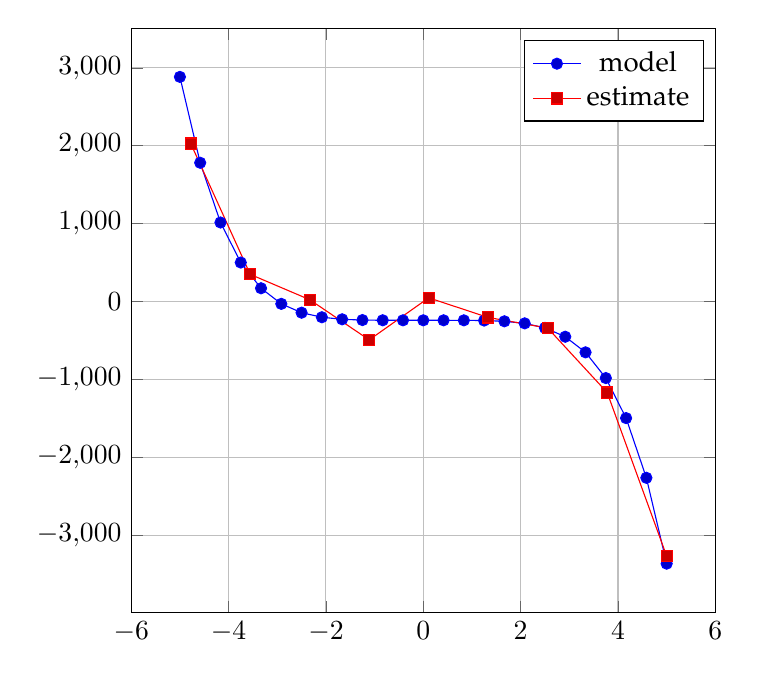
\begin{tikzpicture} \begin{axis}[ height=9cm, width=9cm, grid=major, ] 

\addplot {-x^5 - 242}; \addlegendentry{model} 

\addplot coordinates { (-4.77778,2027.60977) (-3.55556,347.84069) (-2.33333,22.58953) (-1.11111,-493.50066) (0.11111,46.66082) (1.33333,-205.56286) (2.55556,-341.40638) (3.77778,-1169.24780) (5.00000,-3269.56775) }; 
\addlegendentry{estimate} 

\end{axis} 
\end{tikzpicture}
\caption{A tikz plot with a caption}
\label{fig:plot}
\end{figure}

Figure \ref{fig:plot} shows a plot generated with tikz and pgfplots.

%\lipsum[4-5]

\section{Another Section}

\begin{table}
\centering
\begin{tabular}{ l | c || r }
  1 & 2 & 3 \\
  4 & 5 & 6 \\
  7 & 8 & 9 \\
\end{tabular}
\caption{A table with numbers}
\label{tab:numbers}
\end{table}

Numbers are shown in table \ref{tab:numbers}

\lipsum[6-12]
\chapter{Example Chapter Two}

\section{First Section}

\subsection{Subsection One}
%\lipsum[1-3]

\subsection{Subsection Two}

%\lipsum[4-5]

\section{Another Section}

%\lipsum[6-13]






\backmatter
% optional: list of figures
\listoffigures
% optional: list of tables
\listoftables
% optional: list of source code listings
\lstlistoflistings

% your BibTex file
\bibliography{bib/references}


\appendix
% include appendix chapters here

\chapter{Appendix A}
\section{Software Framework Documentation}\label{sec:FrameworkDoc}

%\lipsum[1-2]


\lstinputlisting[language=C++,caption=Example code snippet, label=HelloWorld_listing]{listings/HelloWorld.cpp}


\end{document}
